\subsubection{RNNIP}

\def\figpath{figures/ftag/dips-note/}

Tracks are reconstructed from energy deposits, or hits, in the inner detector system and are required to pass a quality selection: 
each track must have at least 7 hits in the silicon layers (pixel and SCT, where dead sensors are not penalized), 
no more than two missing hits where expected in the silicon layers, 
no more than one hit shared by multiple tracks, 
at least one hit in the pixel detector, and $|\eta| < 2.5$. 

%\subsection{Algorithm overview}

% from dips intro
% The choice of the RNN architecture was motivated by the capability to operate over jets with variable numbers of tracks, while the use of neural networks provided the flexibility to add more information about the track kinematics into the tagging discriminant.
%while avoiding the "curse of dimensionality" inherit when using histograms to build up likelihood templates \cite{papamakarios2019neural}.
%By modelling the jet as a sequence (or an ordered set of tracks) the RNN can operate over an arbitrary number of associated 


RNNs operate on variable length \emph{sequences} by iterating over the sequence elements, processing them with a neural network, and using previously processed elements when processing new ones. 
It then outputs a fixed size vector that can be used for classification. 
The RNNIP algorithm utilizes a Long Short Term Memory (LSTM) cell for the RNN to preserve long range correlations between the elements of the sequence \cite{LSTMs}. 
As shown in \cite{ATL-PHYS-PUB-2017-003}, the accounting for these correlations allows the RNN to be more performant than IP3D even when trained on the same inputs.
The use of neural networks instead of histograms allows one to avoid the "curse of dimensionality" when using additional variables sensitive to the kinematics of the $b$-hadron decay which significantly improve performance \cite{ATL-PHYS-PUB-2017-003}.
%The benefit of using an RNN as opposed to a standard multi-layer perceptron is that the RNN architecture that can operate natively over varying length inputs (i.e, a varying number of tracks in the jet) by sharing weights for the operations that update the hidden states. This allows the RNN to train with fewer parameters to get a similarly performing network \cite{need ref}.


\begin{figure}[htbp]
\centering
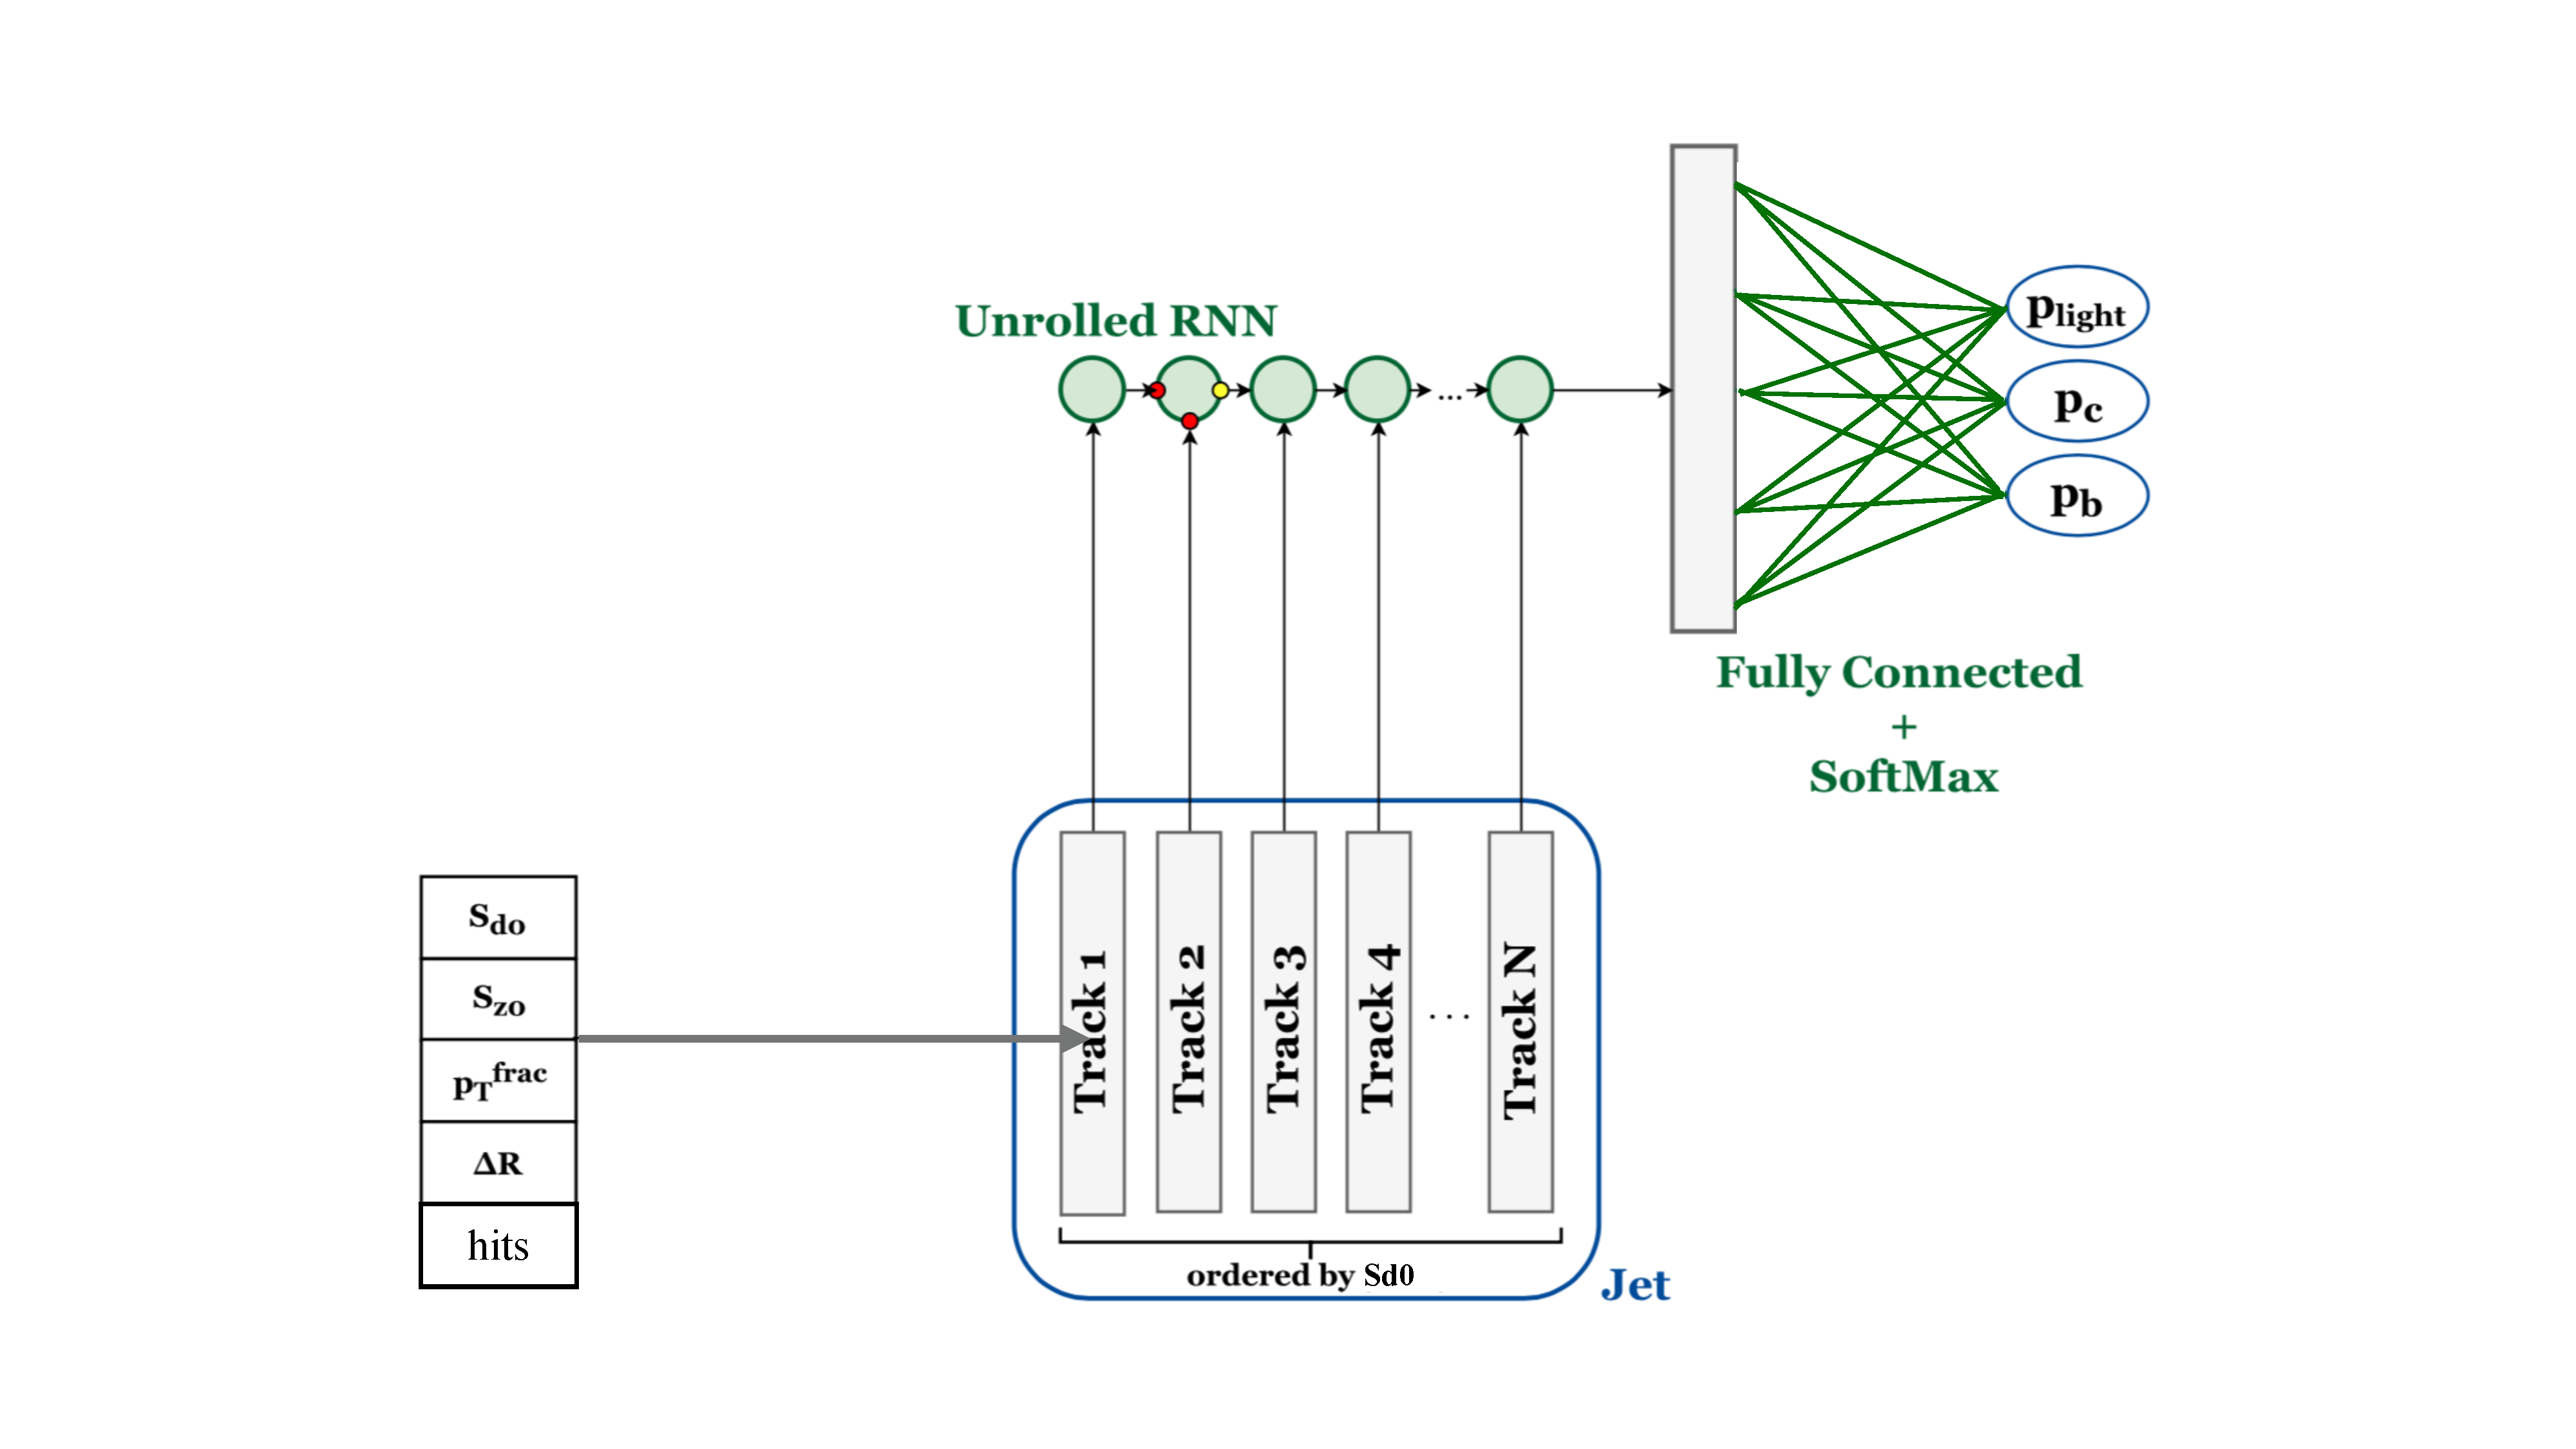
\includegraphics[width=0.8\linewidth]{figures/ftag/RNN-graphic}
\caption{RNNIP architecture (modified from \ref{ATL-PHYS-PUB-2017-003}).}
 \label{fig:RNN-graphic}
\end{figure}


An implementation of the RNNIP algorithm is used as the baseline for comparison to DIPS, but has further optimisations with respect to~\cite{ATL-PHYS-PUB-2017-003}. The RNNIP architecture comprises a 100 dimensional LSTM hidden state and a dropout layer, with dropout fraction of 0.2, before a 20 unit fully connected layer for classification, uses track IP significance, kinematics, and the number of hits in the silicon detectors as features (described in Table~\ref{table:inputs}), and orders the tracks by $s_{d_0}$.
%The RNNIP presented here has some modifications with respect to the one in \cite{ATL-PHYS-PUB-2017-003}. First, since the original RNNIP presentation, significant work has gone into the calibration of the high level tagger, DL1r, which includes as inputs the RNNIP outputs. The measurement of the data-to-MC scale factors in $l$-jets poses a unique challenge since even if we start with a l-jet dominated sample, our $b$-taggers are so powerful that cutting on the $b$-tagging discriminant gives a $b$-jet dominated sample that makes it infeasible to measure the $l$-jet efficiency directly in data. To account for this, we instead design a "flipped" tagger such that the performance on $l$-jets stays the same, but the performance on identifying $b$-jets is dramatically reduced \cite{ATLAS-CONF-2018-006}. Since the large impact parameters for $l$-jets are dominantly from resolution effects, they are mostly symmetric about 0, while the HF tracks from the long lived hadron decay bias the IP distributions in $b$-jets to positive values, as shown in Figure~\ref{fig:flippedInputs}. Therefore, the flipped versions of the RNNIP and IPXD taggers just change the sign of the IP inputs to reduce the $b$-tagging efficiency. The RNNIP presented in \cite{ATL-PHYS-PUB-2017-003} ordered the tracks by an $|s_{d0}|$ sort, but this washes away\footnote{Too informal - when I have data look up ananyms for ameliorate} some of the information we were trying to encode for the flipped tagger. The RNN presented here and in the more recent \cite{PFlowPublicPlots2019} the tracks were therefore ordered by $s_{d0}$ instead. In addition, previously, to be compatible with RNNIP the same inputs were used as the IPXD algorithms by taking the category encoding the track quality in an 2-dimensional embedding before feeding it in as an input to the LSTM. Now we simply feed in the hits variables which went into the IPXD category definitions, which led to an $\mathcal{O}\left(10\%\right)$ improvement for the $l$ rejection at a the 60\% efficiency for identifying $b$-jets.\footnote{Rejection hasn't been defined yet in the note - should I take this number out?} Finally the architecture has been modified. The size of the LSTM hidden state has been increased to 100 for $t\bar{t}$ trainings and 400 for the extended hybrid sample, where the size of the hidden state was optimised for each physics sample. Additionally, in the final layer before classification, a dropout layer has been added with a dropout fraction of 0.2 to improve the network's generalization to the test set \cite{Dropout}, and then the hidden state is fed through a fully connected layer with 20 hidden units before the softmax layer.

%\subsection{Optimizations}


\begin{table}[h!]
  \centering
    \begin{tabular}{l | l } % <-- Alignments: 1st column left, 2nd middle and 3rd right, with vertical lines in between
      \textbf{Input} & \textbf{Description}  \\
      \hline
      \hline
  $s_{d0}$ & $d_0 / \sigma_{d0}$: Transverse IP significance \\
	$s_{z0}$ & $z_0 \sin \theta / \sigma_{z0 \sin \theta}$: Longitudinal IP significance \\
	$\log \pT^{frac}$ & $\log \pT^{track} / \pT^{jet}$: Logarithm of fraction of the jet $\pT$ carried by the track \\
	$\log \Delta R$ & Logarithm of opening angle between the track and the jet axis \\
	IBL hits & Number of hits in the IBL: could be \{ 0, 1, or 2 \} \\
	PIX1 hits & Number of hits in the next-to-innermost pixel layer: could be \{ 0, 1, or 2 \} \\
	shared IBL hits & Number of shared hits in the IBL \\
	split IBL hits & Number of split hits in the IBL \\
	nPixHits & Combined number of  hits in the pixel layers \\
	shared pixel hits & Number of shared hits in the pixel layers \\
	split pixel hits &  Number of split hits in the pixel layers \\
	nSCTHits  & Combined number of hits in the SCT layers \\
	shared SCT hits & Number of shared hits in the SCT layers \\
    \end{tabular}
    \caption{Track features used as inputs for RNNIP and DIPS algorithms.}
    \label{table:inputs}
\end{table}

